% !TEX program = xelatex
\DocumentMetadata{lang=en} % required for transparent package
\documentclass[10pt,aspectratio=169]{beamer}
\newcommand{\subhead}[1]{\flushleft {\bf\large #1}\\}

% remove footcite numbers
\makeatletter
\def\@makefnmark{}
\makeatletter

\setbeamersize{text margin left=5mm,text margin right=5mm} 

\newcommand\focus[1]{%
	{\alert{\textbf{#1}}}
}

\usepackage{amsthm,amsmath,amssymb,braket,fontspec,unicode-math,fontenc,transparent}
\usepackage[absolute,overlay]{textpos}

\graphicspath{{./figures/}}
\usetheme[numbering=none]{focus}
\setmainfont{Lato}
\setsansfont{Hero New}
\setmathfont{Fira Math}

\usepackage[backend=bibtex,url=false,doi=false,style=authoryear]{biblatex}
\setbeamertemplate{bibliography item}{}
\bibliography{bib}
\AtBeginBibliography{\scriptsize}

\setbeamerfont{title}{size=\LARGE\scshape}
\setbeamerfont{author}{size=\Large}
\setbeamerfont{institute}{size=\large}
\setbeamerfont{date}{size=\large}
\setbeamerfont{frametitle}{size=\Large\scshape}
\setbeamerfont{sectiontitle}{size=\small\scshape}
\setbeamerfont{alerted text}{series=\bfseries}

\title{Pseudogapped non-Fermi liquid phase arising from Kondo breakdown at the Mott transition}
\subtitle{What lies between a Fermi liquid and a Mott insulator in 2D?}

\author{Abhirup Mukherjee, Siddhartha Lal}

\institute
{
	Department of Physical Sciences,\\
	Indian Institute of Science Education and Research Kolkata
}
\date{\today}
\titlegraphic{
	\vspace{80pt}
	
\includegraphics[width=0.08\textwidth]{epqm_logo_mod.jpeg}\hspace*{20pt}
\includegraphics[width=0.08\textwidth]{dps_logo.jpeg}\hspace*{350pt}
}

\begin{document}

\begin{frame}
    % Print the title page as the first slide
    \titlepage
\end{frame}

\begin{frame}{Some Questions}
\footcite{keimer2015quantum,ProustTaillefer2019,loeserKapitulnik1996,Norman1998,Hashimoto2014,KyungKotliar2006,MacridinAzevedo2006,WuFerrero2018,anirbanmott2,HilleAndergassen2020}
The anomalous \alert{pseudogap} (PG) phase exhibits nodal-antinodal dichotomy.\\[5pt]

No general consensus yet regarding
\begin{itemize}
	\item its \alert{relation} to the Mott insulating and superconducting phases proximate to it
	\item how it \alert{evolves} from weak-coupling to strong-coupling
	\item whether the \alert{nodal-antinodal dichotomy} is intrinsic
to the model
\end{itemize}

\begin{center}
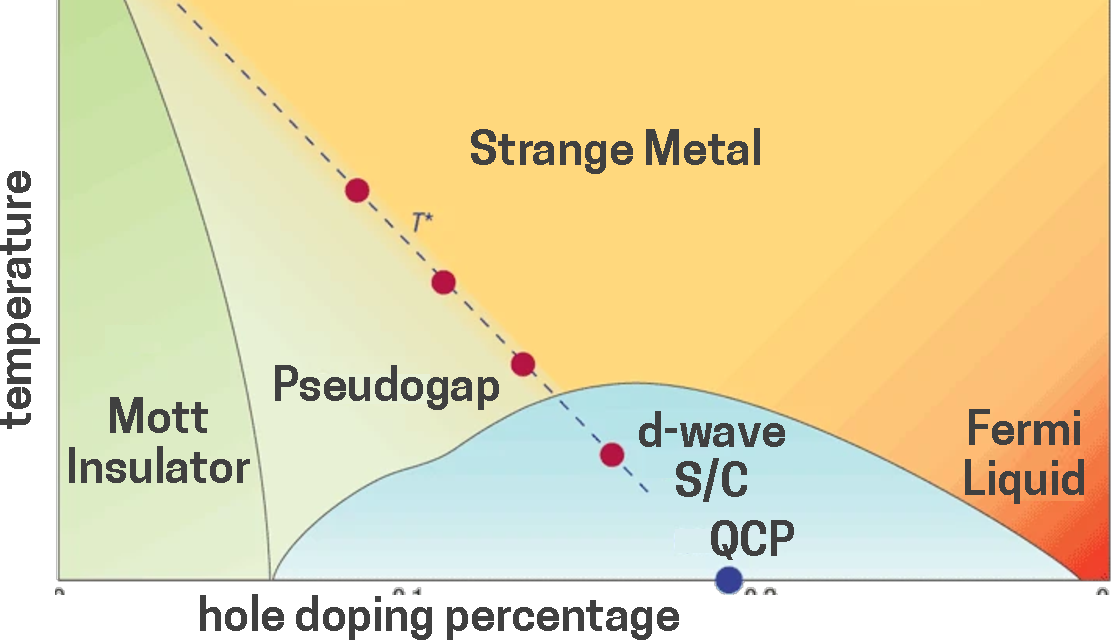
\includegraphics[height=0.2\textwidth]{cuprates.pdf}
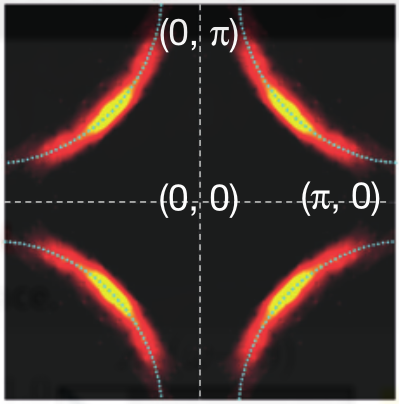
\includegraphics[height=0.2\textwidth]{fermiArc1.png}
\end{center}

\end{frame}

\begin{frame}{A New Auxiliary Model Approach Towards Interacting Models}
	\begin{minipage}{0.4\textwidth}
	1. Solve an appropriate impurity model, \(H_\text{imp}\)
	\begin{itemize}
		\item Lattice symmetry
		\item Impurity phase transition
	\end{itemize}
	\end{minipage}
	\hfill
	\begin{minipage}{0.48\textwidth}
	2. Explicitly construct lattice model by applying manybody translation operators:
	\[ H_\text{latt} = \sum_{\bf r} T^\dagger({\bf r}) H_\text{imp}({\bf r_0})T({\bf r})\]
	\end{minipage}

	\vfill
	\begin{minipage}{0.53\textwidth}
	3. Relate computables across the models,\\ using manybody Bloch's theorem\\[5pt]
	Greens functions: 
	\(\tilde G({\bf K}\sigma; \omega) = G^>(\mathcal{T}^\dagger_{{\bf K}\sigma}, \omega - \varepsilon_{{\bf K}}) + G^<(\mathcal{T}^\dagger_{{\bf K}\sigma}, \omega + \varepsilon_{{\bf K}})\)\\[5pt]
	Equal-time correlation functions:\\
	\(C_{\mathcal{O}}({\bf k}_1,{\bf k}_2) = \sum_{{\Delta}}\braket{{\bf r}_c + {\Delta} | \mathcal{\tilde O}({\bf k}_2) | {\bf r}_c}\braket{{\bf r}_c | \mathcal{\tilde O}^\dagger({\bf k}_1) | {\bf r}_c}\)
	\end{minipage}
	\hfill
	\begin{minipage}{0.45\textwidth}
	where 
	\[G^>(\mathcal{O}^\dagger, t) = -i\braket{\mathcal{O}(t)\mathcal{O}^\dagger}\]
	\[\mathcal{T}_{{\bf K}\sigma} = c_{{\bf K}\sigma}\left(\sum_{\sigma^\prime}c^\dagger_{d\sigma} + \text{h.c.}\right) + c_{{\bf K}\sigma}\left(S_d^+ + \text{h.c.}\right)\]
	\[\mathcal{\tilde O}({\bf r}) = \mathcal{O}({\bf r})\mathcal{O}^\dagger(d)\]
	\end{minipage}
	
	
	
\end{frame}

\begin{frame}{The Core Ingredient: A Lattice-Embedded Impurity Model}
\begin{minipage}{0.75\textwidth}
\begin{equation}\begin{aligned}
	\mathcal{H} = H_\text{cbath} + H_\text{imp-cbath} + H_\text{cbath-int}~,\\
	H_\text{cbath} = -2t\sum_{{\bf k}}\left[\cos(ak_x) + \cos(ak_y)\right] c^\dagger_{{\bf k},\sigma}c_{{\bf k},\sigma}~.\\
	H_\text{imp-cbath} =\frac{1}{2} J\sum_{\sigma_1,\sigma_2}\sum_{Z} {\bf S}_d\cdot c^\dagger_{Z\sigma_1}{ \tau}_{\sigma_1,\sigma_2} c_{Z\sigma_2}~,\\
	H_\text{cbath-int} = -\frac{W}{2}\sum_{Z} \left(n_{Z\uparrow} - n_{Z\downarrow}\right)^2 ~,
\end{aligned}\end{equation}

\begin{equation}\begin{aligned}
	J_{{\bf k}, {\bf k}^\prime} = \frac{J}{2}\left[\cos\left({\bf k}_x - {\bf k}^\prime_x\right) + \cos\left({\bf k}_y - {\bf k}^\prime_y\right)\right] ~,\\
	W_{{\bf k}, {\bf k}^\prime,{\bf q}, {\bf q}^\prime} = W\left[\cos\left({\bf k}_x - {\bf k}^\prime_x + {\bf q}_x - {\bf q}^\prime_x\right) + \cos\left({\bf k}_y - {\bf k}^\prime_y + {\bf q}_y - {\bf q}^\prime_y\right)\right] ~.
\end{aligned}\end{equation}
\end{minipage}
\begin{minipage}{0.2\textwidth}
	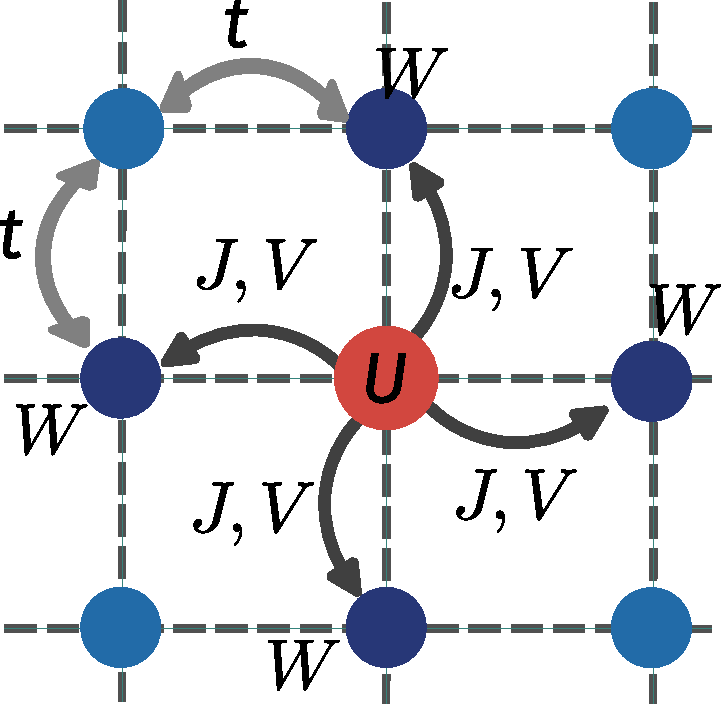
\includegraphics[width=\textwidth]{pWaveEsiam.pdf}
\end{minipage}
\end{frame}

\begin{frame}{Pseudogapping Transition from Kondo Breakdown}
\begin{minipage}{0.48\textwidth}
Unitary RG analysis - integrate out high-energy states in the conduction bath:
\[\Delta J^{(j)}_{{\bf k}_1, {\bf k}_2} = -\sum_{{\bf q} \in \text{PS}} \frac{J^{(j)}_{{\bf k}_2,{\bf q}} J^{(j)}_{{\bf q},{\bf k}_1} + 4J^{(j)}_{{\bf q}, {\bf \bar q}} W_{{\bf \bar q}, {\bf k}_2, {\bf k}_1, {\bf q}}}{\omega - \frac{1}{2}|\varepsilon_j| + J^{(j)}_{{\bf q}}/4 + W_{{\bf q}}/2}\]
\end{minipage}
\begin{minipage}{0.48\textwidth}
	\begin{itemize}
		\item Impurity model shows momentum-anistropic screened phase between SC and LM phases.
		\item Impurity-bath spin correlations show anisotropy
		\item Lattice model DOS shows pseudogap
	\end{itemize}
	
\end{minipage}
	
\begin{center}
    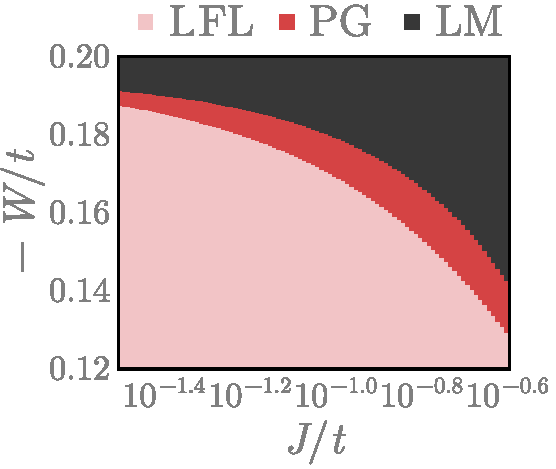
\includegraphics[width=0.32\linewidth]{phaseDiagram.pdf}
    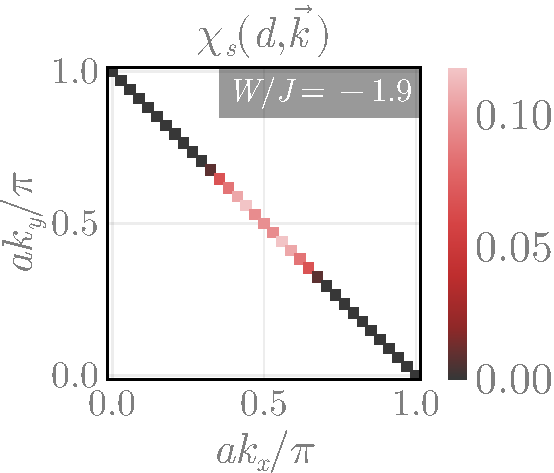
\includegraphics[width=0.32\linewidth]{SF-3.pdf}
    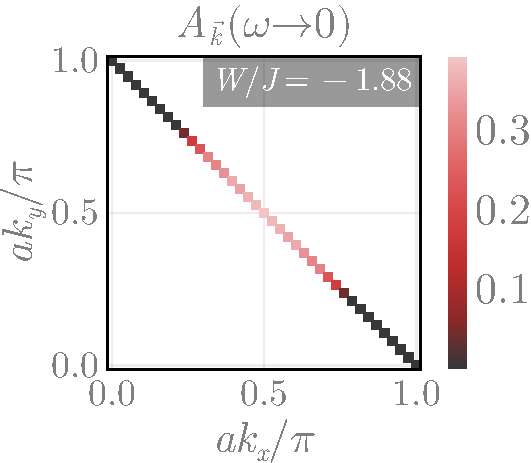
\includegraphics[width=0.32\linewidth]{kspaceDOS-3.pdf}
\end{center}
\end{frame}

\begin{frame}{Unraveling of Kondo screening}
The $k-$space anisotropic nature of the Kondo breakdown process can be visualised in terms of zeros of $J_{{\bf k}_N, {\bf k}}$.
\begin{itemize}
	\item $J_{{\bf k}_N, {\bf k}}$ for ${\bf k}$ close to the adjacent nodes turn RG irrelevant first, and a patch of zeros subsequently appears in $J_{{\bf k}_N, {\bf k}}$ around this point. 
	\item Tuning $W/J$ further extends the patch of zeros in $J_{{\bf k}_1, {\bf k}_2}$ for all ${\bf k}_{1}$ lying between a given node and the nearest antinodes. 
	\item At $W/J=(W/J)_{\text{PG}}$, the antinode joins this connected region of zeros in $J_{{\bf k}_1, {\bf k}_2}$, marking the onset of the PG.
\end{itemize}

\begin{minipage}{0.19\textwidth}
This is an interaction-driven Lifshitz transition of the Fermi surface~\footcite{WuFerrero2018}.
\end{minipage}
\begin{minipage}{0.8\textwidth}
    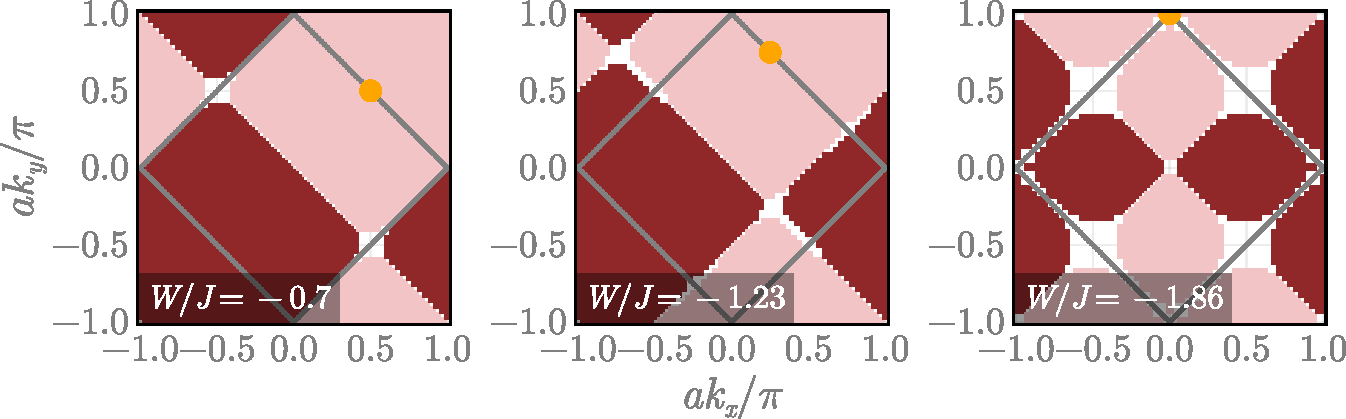
\includegraphics[width=\linewidth]{zerosFlow.pdf}
\end{minipage}

\end{frame}

\begin{frame}{Dynamical Spectral Weight Transfer}
\begin{itemize}
	\item strong fluctuations observed in \alert{charge correlations} between the gapless nodal and gapped antinodal regions in PG regime
	\item PG formation results from the \alert{transfer of spectral weight} from low to high energies
	\item PG coincides with the appearance of poles of the lattice model self-energy $\Sigma ({\bf k},\omega=0)$ near the antinodes
\end{itemize}

\begin{center}
    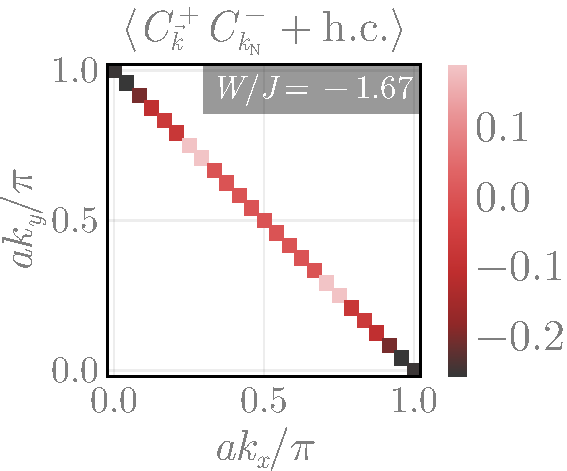
\includegraphics[width=0.38\linewidth]{cfnode-2.pdf}
    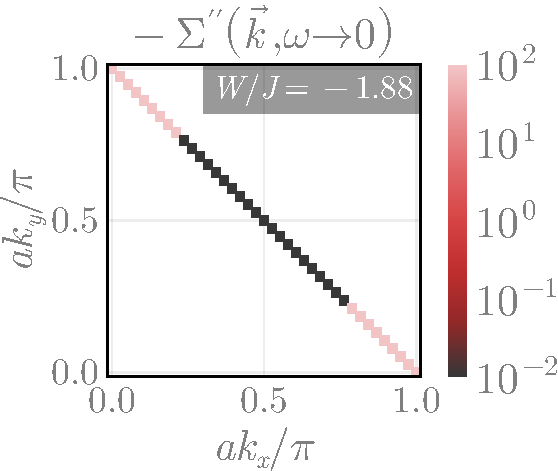
\includegraphics[width=0.38\linewidth]{selfEnergyKspace-3.pdf}
\end{center}
\end{frame}


\begin{frame}{Non-Fermi liquid nature of the pseudogap}
	\begin{itemize}
		\item In PG phase, Kondo processes between adjacent \(k-\)space quadrants are removed at low-energies
		\item Effective \alert{two-channel Kondo} description - each pair of opposite quadrants forms a channel
		\item \alert{Non-Fermi liquid} physics - vanishing quasiparticle residue, and \(\Sigma\) poles near \(\omega=0\)
	\end{itemize}
	
\vspace{-5pt}
\begin{center}
    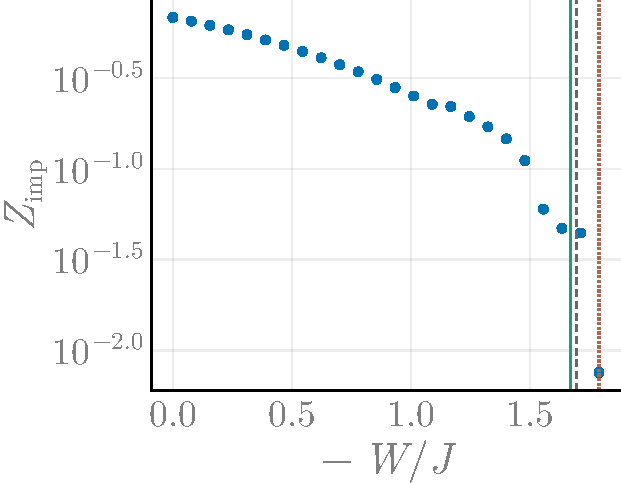
\includegraphics[width=0.4\linewidth]{localQPResidue.pdf}
    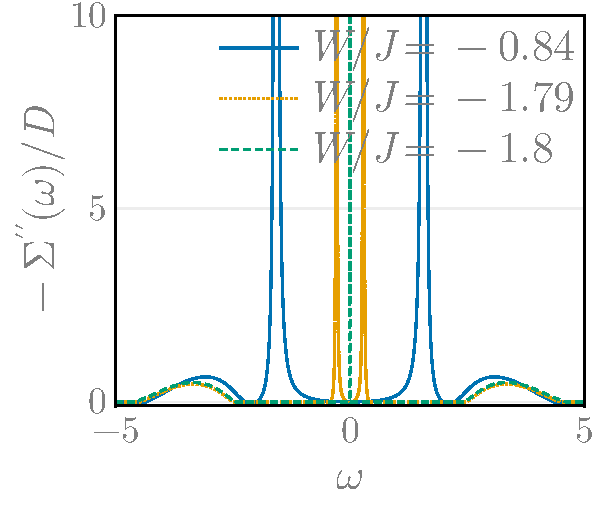
\includegraphics[width=0.4\linewidth]{sigmaImag_49-1000.pdf}
\end{center}
\end{frame}

\begin{frame}{Singular Nodal Metal}

\end{frame}

\begin{frame}{Non-local nature of the pseudogap}
	\begin{itemize}
		\item real-space correlations and entanglement undergo a crossover within the pseudogap from short-ranged to \alert{long-ranged} behaviour
		\item This is further evidence of the \alert{breakdown of local Kondo screening}, and resulting Landau quasiparticle excitations
		\item the Mott transition observed by us for the Hubbard-Heisenberg model on the square lattice lies well beyond the paradigm of \alert{local quantum criticality}
	\end{itemize}

\begin{center}
    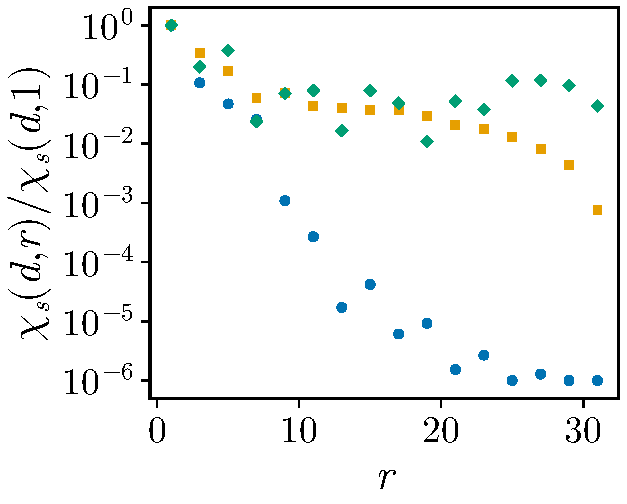
\includegraphics[width=0.35\linewidth]{SF-di_69-2000.pdf}
    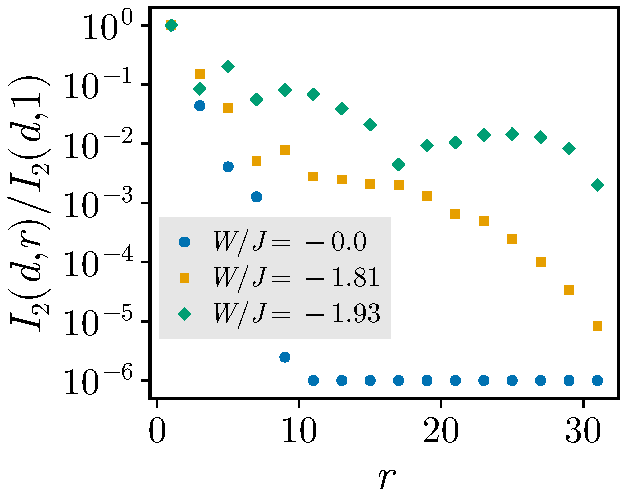
\includegraphics[width=0.35\linewidth]{I2-di_69-2000.pdf}
\end{center}
\end{frame}

\begin{frame}{The Final Slide}
	\alert{Conclusion}
	\begin{itemize}
		\item  we find compelling evidence that the Mott transition on the square lattice involves continuous passage through a pseudogap phase arising from the breakdown of Kondo screening
		\item pseudogap is comprised of gapped antinodal regions in k-space together with an increasingly non-local nodal non-Fermi liquid metal whose excitations lie proximate to a singular Fermi surface
	\end{itemize}

	\alert{Future Directions}
\begin{itemize}
	\item Heavy fermions?
	\item Doping the pseudogap phase - superconductivity?
\end{itemize}

\end{frame}


\end{document}
